
\documentclass[a4paper, 11pt]{article}
%\usepackage[UTF8]{ctex}
\usepackage{amsmath}
\usepackage{amsfonts}
\usepackage{amssymb}
%\usepackage{apacite}
\usepackage{siunitx}
\usepackage{graphicx}
\usepackage{url}
\usepackage{subfigure}
\usepackage{float}
\usepackage{booktabs}
\usepackage{caption}
\usepackage{makecell}
\usepackage{listings}
\usepackage{xcolor}
\usepackage{minted}
\usepackage{geometry}
%\geometry{a4paper,left=2cm,right=2cm,top=1cm,bottom=1cm}
\geometry{a4paper,scale=0.8}

	\title{ASC Student Supercomputer Challenge 2020-2021 Preliminary Round Thesis}
	\author{TOSA ASC}
	\date{2020-12-30}


\begin{document}

	\maketitle
	%\captionsetup[figure]{labelfont={bf},name={Photo.},labelsep=period}
	\captionsetup[figure]{labelfont={bf},name={Figure.},labelsep=period}
	
	%\begin{abstract}
		%[Abstract here. 120 words]
	%\end{abstract}
	
	\pagenumbering{roman}
	\tableofcontents
	\newpage
	\pagenumbering{arabic}
	
	

	\section{Introduction of the university department activities in supercomputing}
		\subsection{Supercomputing-related hardware \& software platforms} 
		
			The High-Performance Computing Public Service of \textit{The Key Laboratory of Embedded System and Service Computing(Tongji University), Ministry of Education} is founded in 2007 In the School of Electronics and Information Engineering of the Tongji University. The service is equipped with IBM P570, Dell PC Servers Cluster, SUN massive storage array. These devices are interconnected as Heterogeneous Computing Platform, providing public services to teaching and researching. The Computing and Analyzing service of the lab, which is equipped with Mini Computers from IBM, and Sugon's x86 Clusters. 
			
			There is an IBM High-Performance Cluster serving for the bio-informatics centre of the School of Life Sciences and Technology, Tongji University, which consists 6 fat nodes(IBM HS22, 2x Intel x5650, 96GB of memory), 30 thin nodes(IBM HS22, 2x Intel x5650, 24GB of memory), DS3200 storage system with 48 2TB Hard Drives. The system is interconnected with QDR 40Gb Infiniband, and its theoretic peak floating performance is 4596.48Gflops. 
		
		
		\subsection{Supercomputing-related courses \& interest groups} 
		
			There are two Supercomputing courses open to undergraduates. One is Supercomputers and Parallel Computing by Ke Sanhuang in the School of Physics. The other one is The Principle and Practice of Parallel Programming by Zhang Yichao in the School of Electronics and Information Engineering. And we have a student club called Tongji Open Source Association. Committed to broaden the horizons of college students, especially for those who is interested in computer knowledge, TOSA give lectures about computer knowledge and advanced technologies frequently, with opportunities to practices by themselves.
			
		\subsection{Supercomputing-related research, applications \\ \& key achievements}
		
			Several teachers in the mentioned lab of the School of Electronics and Information Engineering have been working on field researches. They had undertaken the project \textit{Granular computing and the technique of compiling, debugging and tuning} funded by the 863 Program, \textit{Automatic extraction of program's heterogenous feature and network  heterogenous parallel computation} funded by National Natural Science Foundation of China and several other programs. Certain research results received second prize of 2008 IEEE International Service Contest. 
			
	\section{Team introduction}
		\subsection{Team setup}
		
			Both of our teammates are interested in supercomputing and are from the same club called Tongji Open Source Association. Once we heard the competition, we immediately attention on it. After looking up relevant information and competition introduction on the Internet, we all hope to join in the competition. After several talk on social platform, our team leader select us according to our personal characteristics.
		
		\subsection{Team members} 
		\captionsetup[figure]{labelfont={bf},name={Photo.},labelsep=period}
			
			\begin{figure}[H]
				\centering
				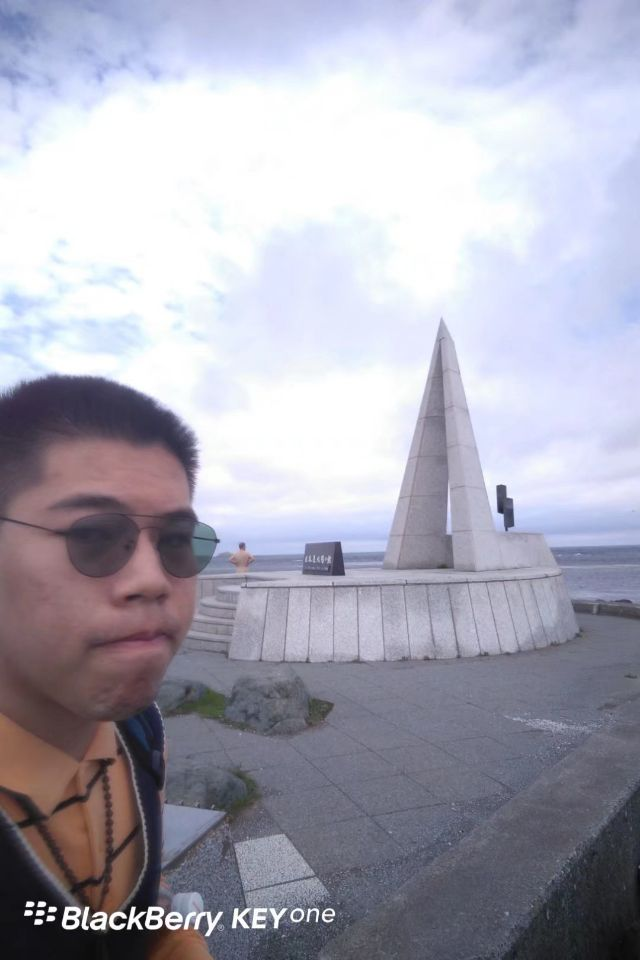
\includegraphics[width=0.3\textwidth]{Lu.jpg}
				\caption{Lu Yan} 
				\label{photo:1}  
			\end{figure} 
			\paragraph{Lu Yan}: intrested in Computational Neuroscience and Neuromorphic Engineering.
			
			
			\begin{figure}[H]
				\centering
				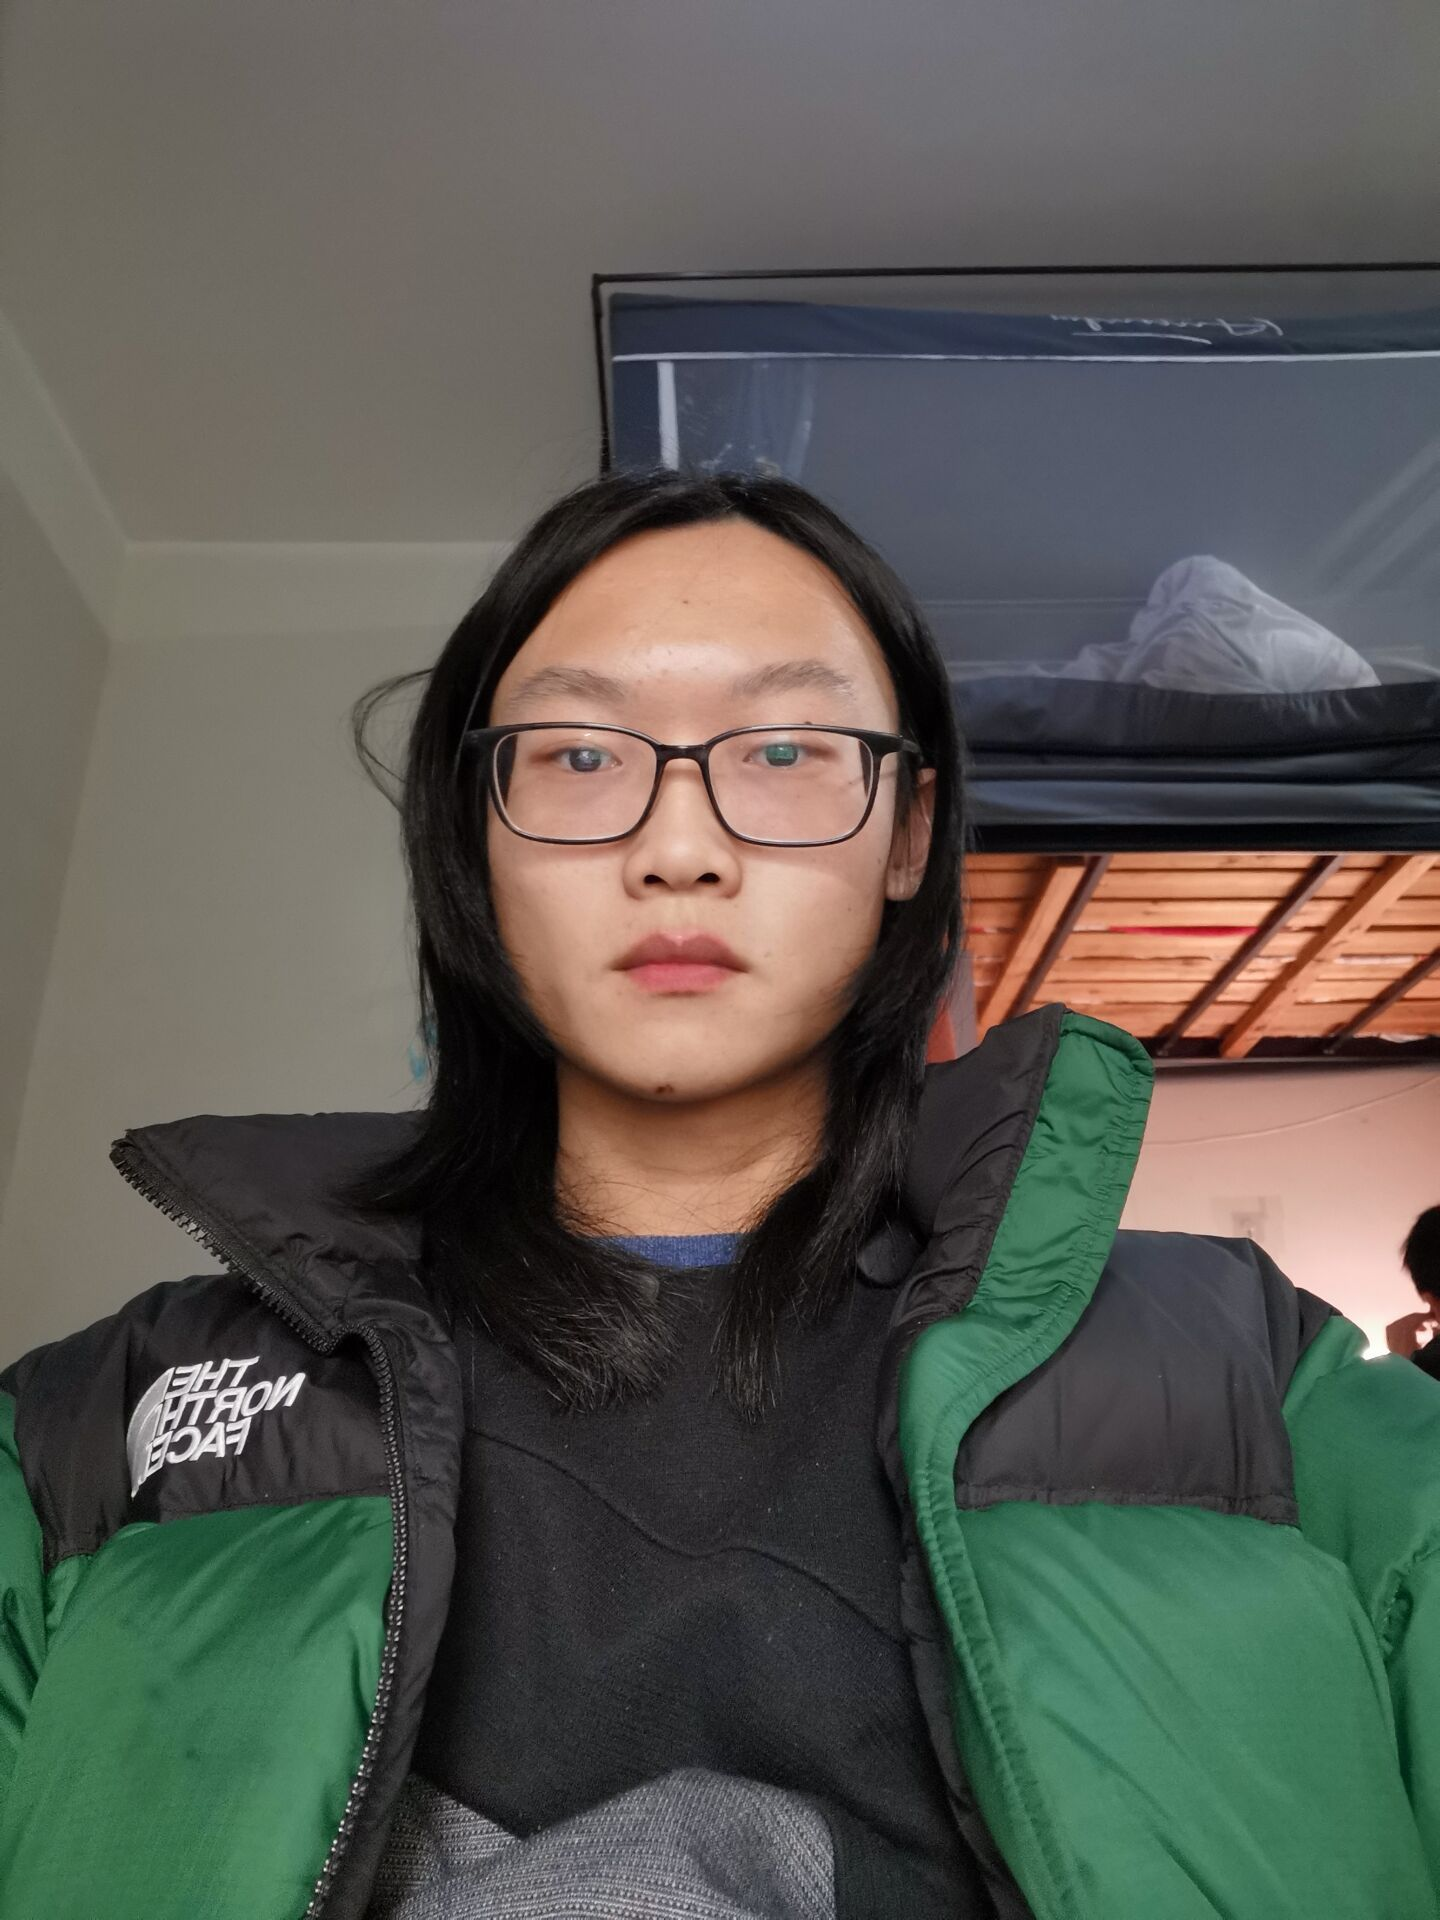
\includegraphics[width=0.3\textwidth]{Liu.jpg}
				\caption{Liu Kongyang} 
				\label{photo:2}  
			\end{figure} 
			\paragraph{Liu Kongyang}: interested in Computer Graphics, Computer Vision and Machine Learning.
			
			
			\begin{figure}[H]
				\centering
				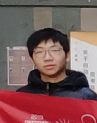
\includegraphics[width=0.3\textwidth]{Qiu.jpg}
				\caption{Qiu Zili} 
				\label{photo:3}  
			\end{figure} 
			\paragraph{Qiu Zili}: interested in Hardware Configuration and Maintainence of HPC.
			
			
			\begin{figure}[H]
				\centering
				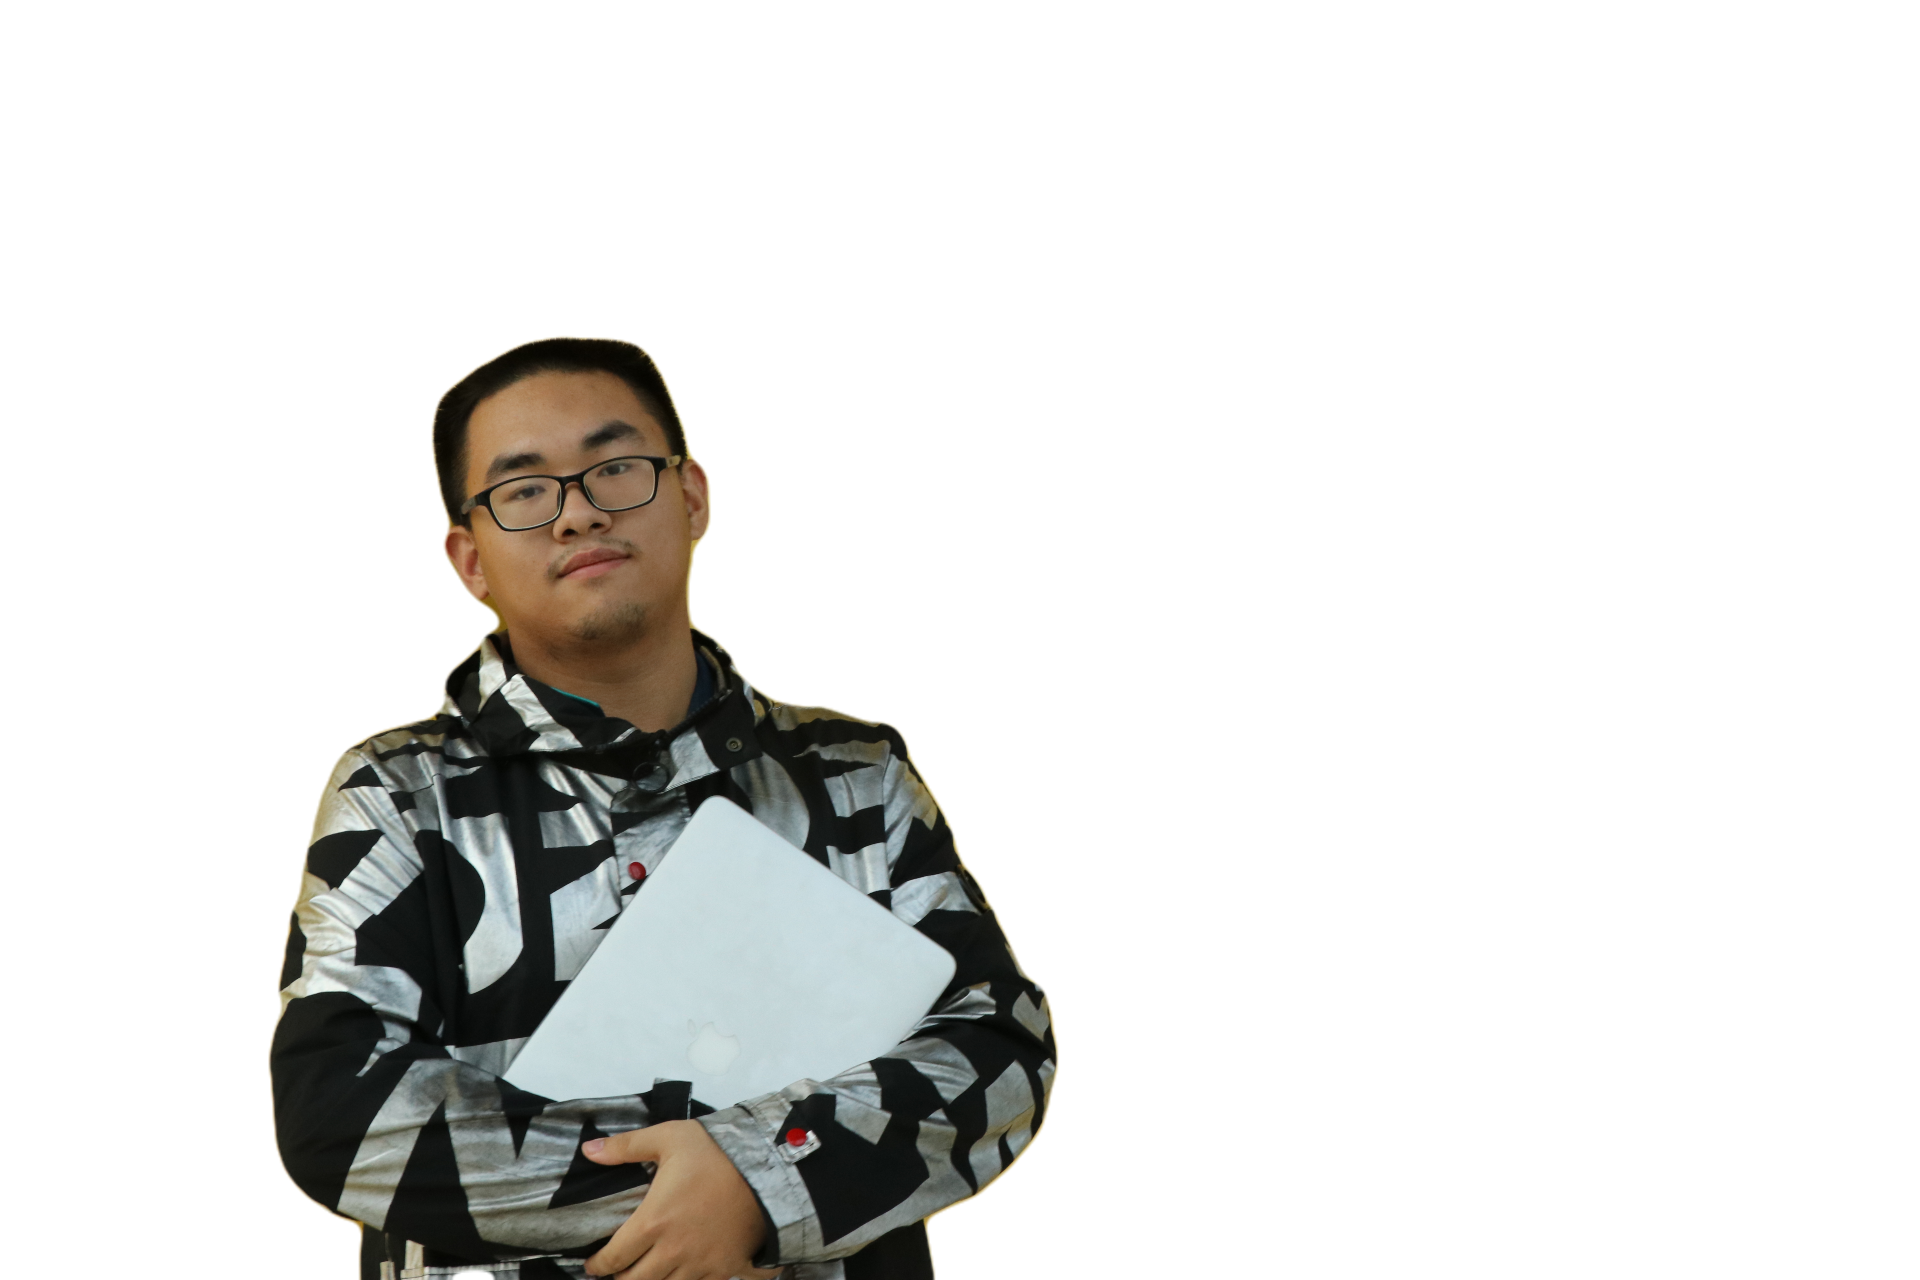
\includegraphics[width=0.3\textwidth]{Jiang.png}
				\caption{Jiang Wenyuan} 
				\label{photo:4}  
			\end{figure} 
			\paragraph{Jiang Wenyuan}: majors in Bioinformatics, and is interested in HPC's application in Biology.
			
			
			\begin{figure}[H]
				\centering
				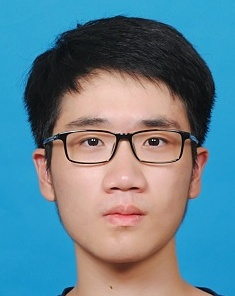
\includegraphics[width=0.3\textwidth]{Xia.jpg}
				\caption{Xia Wenyong} 
				\label{photo:5}  
			\end{figure} 
			\paragraph{Xia Wenyong}: interested in algorithm designation of HPC.
			
		\captionsetup[figure]{labelfont={bf},name={Figure.},labelsep=period}
		\subsection{Team motto} 
		
			The ASC20-21 Team of Tongji University is a brand new one, though we are neither experienced nor with adequate resources, all of us are talented in the art of problem solving, and is eager to embrace the new knowledge on HPC. We'll try our best in each challenge!
		
		
	\section{Technical proposal requirements}

		\subsection{Design of HPC system}
			\begin{table}[H]
				\begin{center}
					\caption{Design of HPC system}
					\label{tab1}  
					\begin{tabular}{l l l}
						\toprule
						Item & Name & Configuration\\			
						\midrule
						Server & \makecell[l]{Inspur \\NF5280M5 \\x6} & \makecell[l]{CPU: Intel Xeon Gold 6230 x2 2.1GHz 20 cores \\ Memory: 32G x12,DDR4,2933Mhz \\ Hard disk: 480G SSD SATA x1 \\ Power consumption estimation:\\ 6230 TDP 125W, memory 7.5W, hard disk 10W}\\
						&&\\
						GPU & Tesla V100 x8 & \makecell[l]{2 of the nodes is equipped with 4 NVIDIA Tesla \\V100.}\\
						&&\\
						HCA card & \makecell[l]{EDR\\
							InfiniBand Mellanox \\ConnectX$^{\tiny{\textregistered}}$-5} & \makecell[l]{HCA card, single port\\
							QSFP, EDR IB\\
							Power consumption estimation: 9W
						}\\
						&&\\
						Cable & InfiniBand cable I & InfiniBand EDR copper cable, QSFP port\\
						&&\\
						Switch & EDR-IB switch & \makecell[l]{Switch-IB$^{\tiny{\texttrademark}}$ EDR InfiniBand switch, \\36 QSFP port\\
							Power consumption estimation: 130W
						}\\
						\bottomrule
					\end{tabular}
				\end{center}
			\end{table}
			There are two modes in theory. When in GPU mode, only two nodes with 4 V100s are used. And when in CPU mode, three nodes are used, but without any load for GPU. 
			
			It is estimated that in GPU mode, $(P_{GPU}+P_{CPU}+P_{Memory}+P_{Hard Disk} )=(8*250+4*125+12*7.5*2+2*10+2*9)=2718W$.
			
			In CPU mode, GPU is all in idle, thus need an estimate of 20W for a single card. For single CPU node, $(P_{CPU}+P_{Memory}+P_{Hard Disk})=(2*125+12*7.5+10+9)=359W$. We use 6 of them, which is 2314W in total. 
			
			Adding 130W to both mode doesn't make it violating power limit.
			
		\subsection{HPL and HPCG}
		\subsubsection{Software and Hardware Environment}
		\begin{table}[H]
			\begin{center}
				\caption{Software and Hardware Environment of our testing platform}
				\label{tab2}
				\begin{tabular}{c l l}
					\toprule
					Item & Name & Configuration\\			
					\midrule
					OS & \makecell[l]{CentOS Linux 8} & \makecell[l]{Kernel: 4.18.0-193.14.2.el8\_2.x86\_64\\
						Shell: bash 4.4.19
					}\\
					&&\\
					GPU & Tesla K80 x2 & \makecell[l]{The node is equipped with 2 NVIDIA Tesla K80.}\\
					&&\\
					CPU & \makecell[l]{Intel\\(Engineering Sample)} & \makecell[l]{Two Engineering Samples of\\ Intel$^{\tiny{\textregistered}}$ Xeon$^{\tiny{\textregistered}}$ Gold 5117 Processor\\ where each core is assigned two processes,\\ a total of 28 cores and 56 processes.}\\
					&&\\
					Libraries & \makecell[l]{CUDA, MKL \\and OpenMPI} & \makecell[l]{CUDA 10.2,\\ Intel$^{\tiny{\textregistered}}$ MKL 2018.0.128,\\OpenMPI 3.2.1}\\
					&&\\
					Complier & \makecell[l]{GCC} & \makecell[l]{GCC version 8.3.1 20191121 (Red Hat 8.3.1-5)}\\
					&&\\
					Memory & 63895MB & \makecell[l]{DDR4 2133MHz}\\
					\bottomrule
				\end{tabular}
			\end{center}
		\end{table}
		\subsubsection{Detailed Configurations} You can find detailed configurations in the attachments.
		\subsubsection{Performance Evaluation} 
			We use GPUs to finish the whole tasks. In theory, a single Tesla K80 can achieve a FP32 (float) performance of 4.113 TFLOPS and a FP64 (double) performance of 1,371 GFLOPS (1:3). We used FP64 to finish these tasks. In theory, the peak performance is 2742 GFLOPs. 
			
			When it comes to HPL, we found 7.131e+02 GFLOPS, that is, 713.1GFLOPS. The efficiency is around 26\%.
			
			When it comes to HPCG\cite{dongarra2016high}, we found 49.3GFLOPS, 69.9GFLOPS, 64.3GFLOPS and 62.2GFLOPS in four subjects. That is around 3\% of the theoretical peak performance.
			
			It's interesting that our HPL/HPCG \% of peak is higher than expected. We have seen at least more than 5\%, sometimes more than 8\%. That may be caused by the low efficiency on HPL, but taking 70\% of peak performance and we have seen a 2-3\% value.
		
		
		
		
		
		
		
		
		\subsection{Language Exam (LE) Challenge}
			\subsubsection{Hardware and Software Environment}
			
				The code is written tested on a Surface Book 2 with 16GB of RAM, i7-8650U and GTX 1060 6G version. A pytorch on Windows 10 under anaconda was deployed, and the CUDA version is 10.1. 
				Because of the lack of Video Memory, we can't train the model even when batch\_size was 4. Thus, we implemented tuning in the given code, and taking data parallelism into consideration. but because of the lack of time and sufficient computing power, it's hard for us to do meaningful training.
				
			\subsubsection{Details}
			
				In this part, we directly import the BERT\cite{devlin2018bert} model from the internet, and deploy it to infer the masked words in the exam. The average accuracy on train is estimated to be more than 60\%. 
				BERT - Bidirectional Encoder Representation from Transformers is issued by Google. It masks tokens randomly when training, and attempts to maximize the conditional probability of certain words in the context. We use this feature to directly infer words from the given context, and choose the most likely one of the four choices. It's a simple but working strategy. 
				
			\subsubsection{The Directory Structure}
				In the \texttt{LE} directory, a test folder and a \texttt{script} folder can be found. The missing model folder has been explained above. In the \texttt{test} folder, an \texttt{answer.json} should be found, which contains the result of test dataset. In the \texttt{script} folder, an \texttt{main.py} should be found, which contains our main program. 
				
		\subsection{The QuEST Challenge} 
		
			\subsubsection{Hardware and Software Environment}
			
				The hardware and software configuration we employed to test our QuEST Challenge is the same as shown in Table \ref{tab2}, and you can find detailed configurations in our attachments.

			\subsubsection{Details}
			
				We first cloned the QuEST\cite{jones2019quest} repository to our testing platform and followed the instructions given in \texttt{README.md} to build the GHZ\_QFT and random circuits. We compiled the \texttt{GHZ\_QFT.c} and \texttt{random.c} with default flags \texttt{-DGPUACCELERATED=0} and \texttt{-DGPUACCELERATED=0}.
				
				After successfully compiling and running the QuEST tasks, we compared the generated \texttt{probs.dat} and \texttt{stateVector.dat} with the corresponding reference data files, and we found no difference, which indicates that the complier and gave out the binary that produces correct results.
				
				Then we tried to employ the Tesla K80 to accelerate the computation. We set the complier flag \texttt{DGPUACCELERATED} to \texttt{-DGPUACCELERATED=1} and configured environment variables to compile a CUDA based QuEST binary. Considering that Tesla K80 have a CUDA \texttt{Compute Capability = 3.7}, another flag \texttt{-DGPU\_COMPUTE\_CAPABILITY=30} is added. The complier gave no warnings or errors, as is expected.
				
				However, when running both tests, only one of the two GPUs is used, and due to the fact that one K80 core has only 12GB of Video Memory but the GHZ\_QFT circuit and random circuit require at least 16GB of Video Memory, we fail to run the simulation at full scale. We cut the circuits to 27 qubits to suit our 12GB of Video Memory and did the same computation under a CPU environment to verify our the results given by GPU. The results given by CPU and GPU are the same, and using GPU only took 10\% to 20\% of the time on CPU platform. Since the results are not the full scale (30 qubits) of the GHZ\_QFT circuit and random circuit, we did not include them in our attachments.
				
				We also tried to compile the MPI version of CPU and GPU based QuEST. The CPU MPI version compiles well, but unfortunately, the  version of QuEST did not support running on multiple GPUs. Since we only had one testing platform, the results of MPI version are almost the same of non-MPI version, so we did not include the results of MPI version in our attachments.
				
				The files in our attachments shows that running on our 28 core CPU, both full scale GHZ\_QFT circuit and random circuit took about 500 seconds to give out desirable results.

			
			\subsubsection{Fine tuning plan}
				
				We plan to fine tune the QuEST Challenge based on following ideas:
				
				\begin{enumerate}
					\item In CPU mode, making full use of the new features provided by Intel in their Xeon$^{\tiny{\textregistered}}$ Scalable$^{\tiny{\textregistered}}$ Processors is necessary to improve the performance. For example, \texttt{AVX512} instruction set should be used and the features of Intel MKL together with Intel C++ Compiler should be integrated.
					\item Using multiple GPU to do the computation is a must in large scale quantum simulations. Trying to bring CUDA and MPI together may be a way to improve the performance and scalability greatly.
				\end{enumerate}

		\subsection{The PRESTO Challenge} 
		
			\subsubsection{Hardware and Software Requirement}
			
				The hardware and software configuration we employed to test our PRESTO Challenge is the same as shown in Table \ref{tab2}. FFTW and OpenMPI are build from source. 

			\subsubsection{Details}
			
				We cloned the PRESTO repository directly and follow the INSTALL instructions As we only have single computer, and GPU Acceleration is not implemented in PRESTO, we directly run given command with built-in timer ’time’. 
				
				Time logged is ‘real 1m10.546s user 1m12.584s sys 0m27.183s’ in task 1 and ‘real 6m40.776s user	6m33.995s sys 0m35.890s’ in task 2. CPU Usage is merely 141\% in task1 and 107\% in task2. More than 1 core is used. However, multi-thread performance is still not optimized enough, since there are 56 threads available. 
			
			\subsubsection{Fine Tuning Plan}
				
				Since PRESTO officially only has CPU support, main attention should be paid to internal multi-thread support and AVX-family instruction sets. If time is efficient, porting to GPU is possible, but not a must. 
				
			
	\section*{Acknowledgement} We thank our teachers, parents, room-mates and girlfriends for their support our taking of the ASC Challenge and tolerance of the noise of our testing platform.

\bibliographystyle{acm}
\bibliography{ref}

\end{document}
